\chapter{波动}
\thispagestyle{empty}
\section{行波}
\par \dy[行波]{XB}
\par 设坐标原点处的质元的运动函数为$y_u=f(t)$,则这一运动沿$x$轴传播时形成波的波函数为
\margin{其中的负号和正号分别对应于沿$x$轴正向和$x$轴负向传播的波.}
\begin{equation}
\eq[y = f(t \mp \frac{x}{u})]
\end{equation}
在给定时刻$t$,$y$为$x$的函数,其图形为叫波形曲线。波的传播表现为波形曲线以波速$u$平移。\jg

\margin{\\ \kg 横波和纵波是弹性介质内波的两种基本形式。但是,不管是横波还是纵波,都只是扰动的传播,介质本身并没有发生沿波方向的迁移。}
\par \dy[横波]{HB} 在扰动中质元的运动方向和绕动的传播方向垂直的波。横波在外形上有峰有谷。\jg

\par \dy[纵波]{ZB} 扰动中质元的运动方向和扰动的传播在一条直线上的波。纵波形成时,介质的密度发生改变,时疏时密。

\section{简谐波}
\dy[简谐波]{JXB} 
\par 原点处质元作简谐运动形成的波为简谐波,其波函数为
\margin{\\[2.5em] \kg 其中的负号和正号分别对应于沿$x$轴正向和$x$轴负向传播的波.}
\margin{\\[1em] 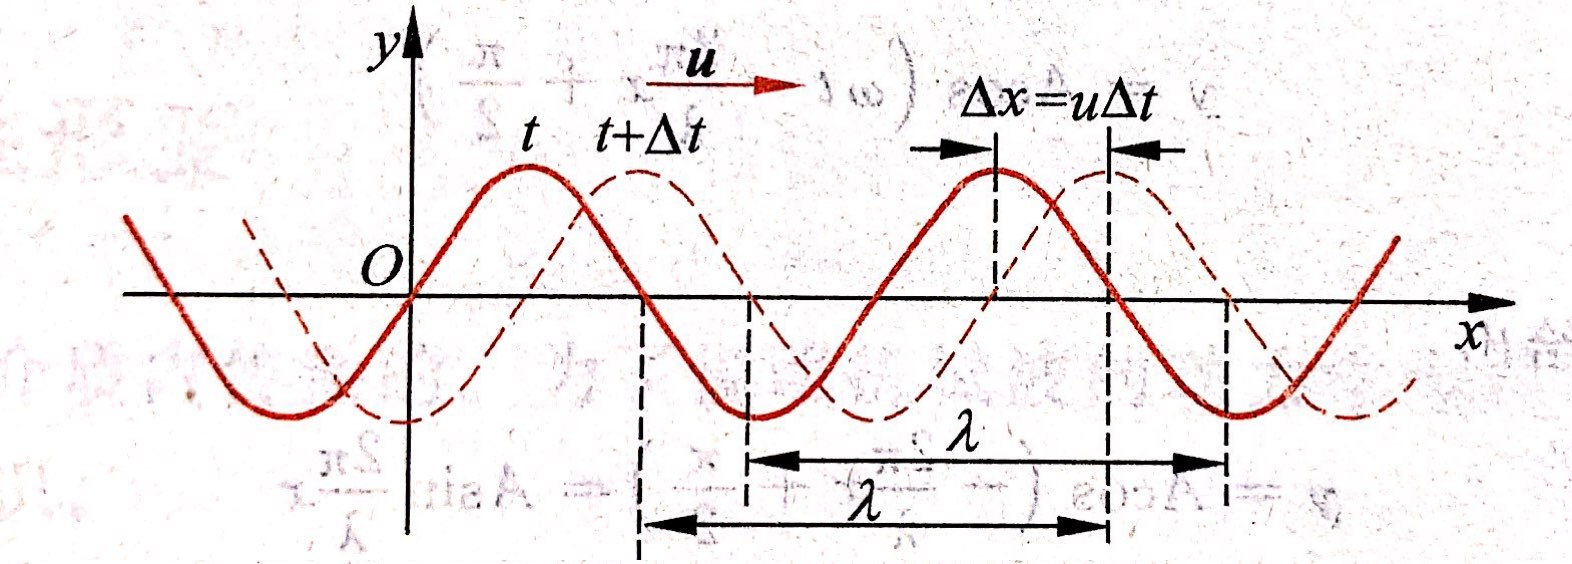
\includegraphics[width=1.2\linewidth]{picture/波1.jpg}}
\begin{equation}
\begin{split}
y&=A\cos\left[ \omega \left( t \mp \frac{x}{u}\right) \right]\\
&= A\cos\left[ 2\pi  \left( \nu t \mp \frac{x}{\lambda}\right) \right]\\
&=A\cos(\omega t \mp kx)
\end{split}
\end{equation}
其中,$k$为波速,$u$为相速度,
\begin{equation}
k=\frac{2\pi }{\lambda},\,\,u=\lambda \nu=\frac{\lambda }{T}
\end{equation}

\section{弹性介质中的波速}
波的形式满足以下方程(一维弹性介质中的横波) 
\begin{equation}
G\frac{\partial^2 y}{\partial x^2}=\rho \frac{\partial^2 y}{\partial t^2}
\end{equation}
代入波的表达式可得波速决定于介质的弹性和密度$\rho $,如\jg

\par \dya[各向同性介质中横波波速]
\margin{\\[1em] \kg $G$为剪切模量\\ \kg $\rho$ 为密度}
\begin{equation}
u=\sqrt{\frac{G}{\rho}}
\end{equation}

\par \dya[各向同性介质中纵波波速]
\margin{\\[1em] \kg $E$为杨氏模量\\ \kg $\rho$ 为密度}
\begin{equation}
u=\sqrt{\frac{E}{\rho}}
\end{equation}

\par \dya[液体、气体中纵波波速]
\margin{\\[1em] \kg $K$为体弹模量\\ \kg $\rho$ 为密度}
\begin{equation}
u=\sqrt{\frac{K}{\rho}}
\end{equation}

\par \dya[拉紧的绳中的横波波速]
\margin{\\[1em] \kg $F$为绳中张力\\ \kg $\rho_l$ 为线密度}
\begin{equation}
u=\sqrt{\frac{F}{\rho_l}}
\end{equation}

\par \dya[气体中声波波速]
\margin{\\[0.5em] \kg $\gamma$为气体比热比\\ \kg $R$ 为普适气体常量}
\begin{equation}
u=\sqrt{\frac{\gamma\,RT}{M}}
\end{equation}

\section{简谐波的能量}
\dy[简谐波的能量]{JXBDNL} 任一质元的动能和弹性势能同相变化。
\begin{equation}
\Delta W_k =\Delta W_p = \frac{1}{2}\Delta W= \frac{1}{2} \rho \omega^2A^2\Delta V\sin^2\left[ \omega (t-\frac{x}{u})\right] 
\end{equation}

\par \dy[能量密度]{NLMD}
\begin{equation}
\omega = \frac{\Delta E}{\Delta V}= \rho \omega^2A^2\sin^2\left[ \omega (t-\frac{x}{u})\right] 
\end{equation}

\par \dy[平均能量密度]{PJNLMD}
\begin{equation}
\overline{\omega }=\frac{1}{2}\rho \omega^2A^2
\end{equation}

\par \dy[波的强度]{BDQD}
\begin{equation}
I=\frac{\overline{P}}{S}=\overline{\omega } u=\frac{1}{2}\rho \omega^2A^2u
\end{equation}

\section{惠更斯原理}
\margin{利用惠更斯原理可以证明波的反射定律和折射定律,并说明波的速度和折射的关系.}
\dy[惠更斯原理]{HGSYL}
介质中波阵面上各点都可看做子波波源,其后任一时刻这些子波的包迹就是新的波阵面。

\section{驻波}
\dy[驻波]{ZB}\jg
\par 两列频率、振动方向和振幅都相同而传播方向相反的简谐波叠加形成驻波,其表达式为
\begin{equation}
y=2A\cos \frac{2\pi x }{\lambda}\cos \omega t 
\end{equation}
驻波实际上是稳定的分段振动,有波节和波腹。\jg

\par \dy[波腹]{BF} 对应使$\displaystyle  \left| \cos \frac{2\pi x }{\lambda} \right| = 1$即$\displaystyle \frac{2\pi x }{\lambda} = k\pi $的各点,因此波腹的位置为
\begin{equation}
x=k\,\frac{\lambda }{2}\,\,\, k = 0, \pm 1,\pm 2, \cdots
\end{equation}

\par \dy[波节]{BJ} 对应使$\displaystyle  \left| \cos \frac{2\pi x }{\lambda} \right| = 0$即$\displaystyle \frac{2\pi x }{\lambda} = (2k+1)\frac{\pi }{2}$的各点,因此波节的位置为
\begin{equation}
x=(2k+1)\,\frac{\lambda }{4}\,\,\, k = 0, \pm 1,\pm 2, \cdots
\end{equation}

\par 两端固定的弦的振动就是驻波。由于两个端点固定不动,所以弦的两端必为波节,故波长只可能是
\margin{\\[0.5em] \kg $L$是弦长.}
\begin{equation}
\lambda_n=\frac{2L}{n}\,\,\,n=1,2,3,\cdots
\end{equation}
\margin{\\[0.5em] \kg $u$是波速.}
而振动的频率只可能是
\begin{equation}
\nu_n=\frac{nu}{2L}\,\,\,n=1,2,3,\cdots
\end{equation}
\par 由上面的式子可以知道,\margin{乐器的弦的振动是基频振动和一些振幅各异的谐频振动的叠加.}在有限的介质中(两端固定的弦线)的驻波波长是量子化的,即只可能取一些分立的值。$n=1$的频率称为基频,$n=2,3,\cdots $的频率称为二次、三次……谐频。

\section{机械波实例}
\dy[声波]{SB}声级
\begin{equation*}
L=10\lg \frac{I}{I_0} \,\,(\rm{dB}),\,\,\,\, I_0=10^{-12} \,\,\rm{W}/\rm{m}^2
\end{equation*}

\dy[地震波]{DZB}有P波、S波、表面波之别。里氏地震级$M$与该次地震释放的能量$E$的关系为
\begin{equation*}
M=0.67 \lg E -2.9
\end{equation*}

\dy[水面波]{SMB}重力波的浅水波速$u=gh$,深水波速$u=\sqrt{g\lambda/2\pi}$.

\section{多普勒效应}
\dy[多普勒效应]{DPLXY}\jg 
\par 接收器接收到的频率有赖于接收器$(R)$或波源$(S)$运动的现象。\jg

\par \dya[波源静止]
\margin{\\ \kg 接收器向波源运动时$v_R$取正值}
\begin{equation}
\nu_R=\frac{u+v_R}{u}\nu_S
\end{equation}

\par \dya[接收器静止]
\margin{\\ \kg 波源向接收器运动时$v_S$取正值}
\begin{equation}
\nu_R=\frac{u}{u-v_S}\nu_S
\end{equation}

\par \dya[接收器、波源均不静止]
\begin{equation}
\nu_R=\frac{u+v_R}{u-v_S}\nu_S
\end{equation}

\par \dya[光学多普勒效应] 决定于光源和接收器的相对运动。
\margin{\\ \kg $v$为光源和接收器的相对运动速度,两者相互接近时$v$取正号.}
\begin{equation}
\nu_R=\sqrt{\frac{c + v}{c - v}}\nu_S
\end{equation}

\par \dy[马赫锥半顶角$\,\,\bm{\alpha}$]{MHZBDJ}\jg 
\par 当波源速度超过它发出的波的速度时,在介质中会产生冲击波,最前面的波面为以波源为顶点的圆锥面。此马赫锥的半定角为
\begin{equation*}
\alpha = \arcsin\frac{u}{v_S}
\end{equation*}

\section{波动方程与振动方程}
在简谐波方程
\begin{equation*}
y =A\cos(\omega t \mp kx)
\end{equation*}
\par 若$x$取固定的值$x=x_0$,那么
\begin{equation*}
y =A\cos(\omega t \mp kx_0) \quad  \Longleftrightarrow \quad y =A\cos(\omega t \mp \varphi_0) \,\,\,(\varphi_0=kx_0)
\end{equation*}
即这个是质点在$x=x_0$的振动方程,画出来的曲线为振动曲线。\jg\jg
\par 若$t$取固定的值$t=t_0$,那么
\begin{equation*}
y =A\cos(\omega t_0 \mp kx) \quad  \Longleftrightarrow \quad y =A\cos(\varphi_0\mp kx) \,\,\,(\varphi_0=\omega t_0)
\end{equation*}
即这个是质点在$t=t_0$的波动方程,画出来的曲线为波动曲线。

\section{波动方程与振动方程的求法}
主思想:固定某一个变量$(x=x_0\,\,/\,\,t=t_0)$后求出振动方程或波动方程,再利用题目所给条件和所学公式求出相关量和相位差即可.\jg
\par \dya[例1] 一简谐波以0.8m/s的速度沿一长弦线传播。在$x=0.1$m处,弦线质点的位移随时间的变化关系为$y=0.05\,\sin (1.0-4.0t)$.求波函数.\jg\jg 
\par 解:由
\begin{equation*}
y=0.05\,\sin (1.0-4.0t),\quad u=0.8\,\text{m/s}
\end{equation*}
可以求出
\begin{equation*}
\omega = 4.0\,\,\rm{s}^{-1},\quad \lambda = \frac{2\pi u}{\omega}=0.4\pi \rm{m}
\end{equation*}
任意$x$处的质元振动的相和$x=x_0$处的相之差为
\begin{equation*}
\Delta \varphi = \frac{2\pi (x-x_0)}{\lambda}=5x-0.5
\end{equation*}
所以波函数为
\begin{equation*}
y=0.05\,\sin (1.0-4.0t+\Delta \varphi )=0.05\,\sin (5x-4.0t+0.5 )
\end{equation*}